\section{Fabrication}
\label{sec:fab}
The object to be printed should be solid, i.e. we have to fill in the inner space of the object with materials as well.
In our method, we use the Zometool structure to fill in most of the inner spaces, while still retaining minimum thickness of the outer shell due to the common setting of 3D printers.
% Note that the thickness might change across different 3D printers.
% However, the input mesh just have the outer surface, and the valid pieces will have both outer and inner surface for 3{D} printer. 
% After we have the inner surface, the pieces have to connect to the Zometool structure. After the process we can get all pieces let can be fabricated, and then we assemble them by connecting to the optimized Zometool structure.
% In order to generate fabricatable shape, it is practical to leave a minimum thickness of the outer shell, and this thickness differs from each printer.
Thus, we prepare the object to be fabricated by generating a inner surface with a predefined thickness, and attach connectors on this inner surface to combine the inner and outer structure.
% and the remaining operations are performed within this inner surface.
    
\subsection{Inner surface}
There are many potential ways to generate inner surface. 
The simplest method is that shrinking the mesh along the vertex normals.
However, it sometimes generate the surface with flipped triangles that stick out of the outer surface (\figname~\ref{fig:shrink_mesh} (b)).

\begin{figure}[ht]
\centering
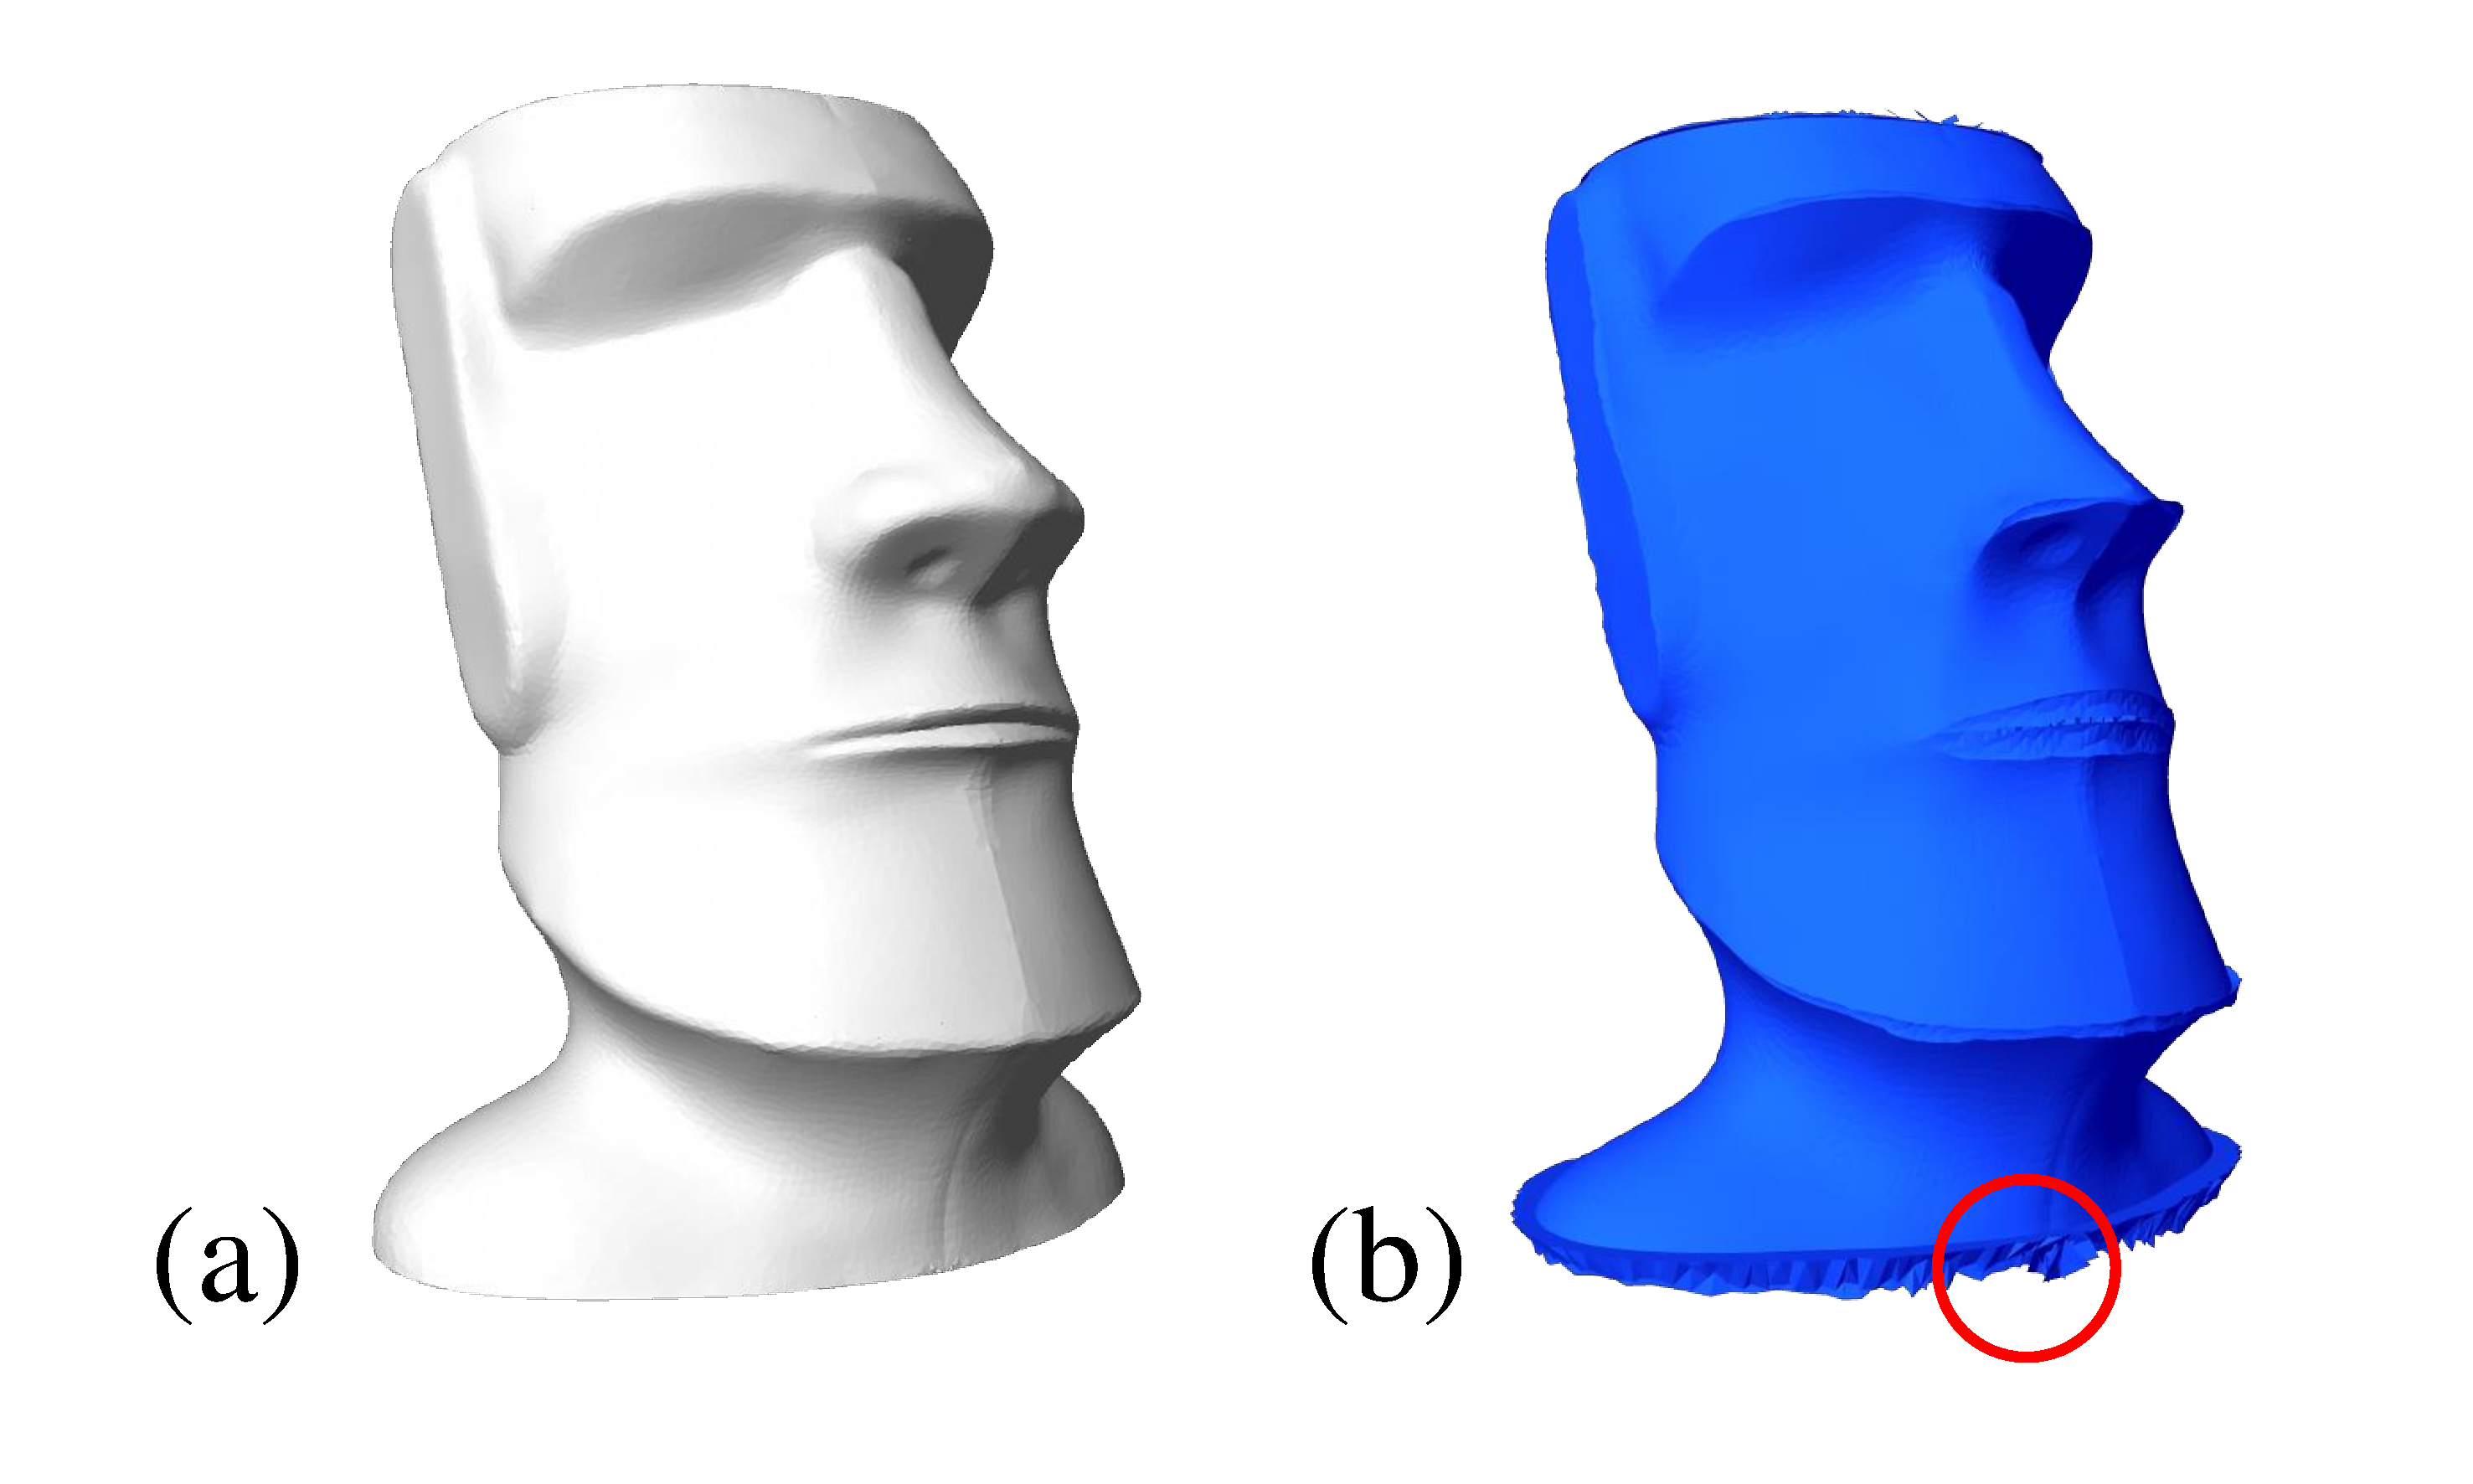
\includegraphics[width=1.0\linewidth]{figs/Shrink_mesh.pdf} 
\caption{
\ichao{Think about if we still need this figure.}
(a) Original mesh (b) Shrunken mesh. Shrink the mesh along the vertex normals is the simple method, but sometimes the mesh will be broken.}
\label{fig:shrink_mesh}
\end{figure}
To prevent this problem, we instead voxelize the original object, and remove the voxels that cover the original surface.
And we use the outer surface of the remaining voxels as our inner surface (\figname~\ref{fig:inner_surface}).
% use the voxelized mesh to handle it. 
% First, we voxelize the original mesh. 
% Then, we choose the outer surface of the voxelized result and combine the original mesh to get the new mesh which has outer and inner surface. 
% The inner surface generation process is illustrated in \figname~\ref{fig:inner_surface}.

\begin{figure}[ht]
\centering
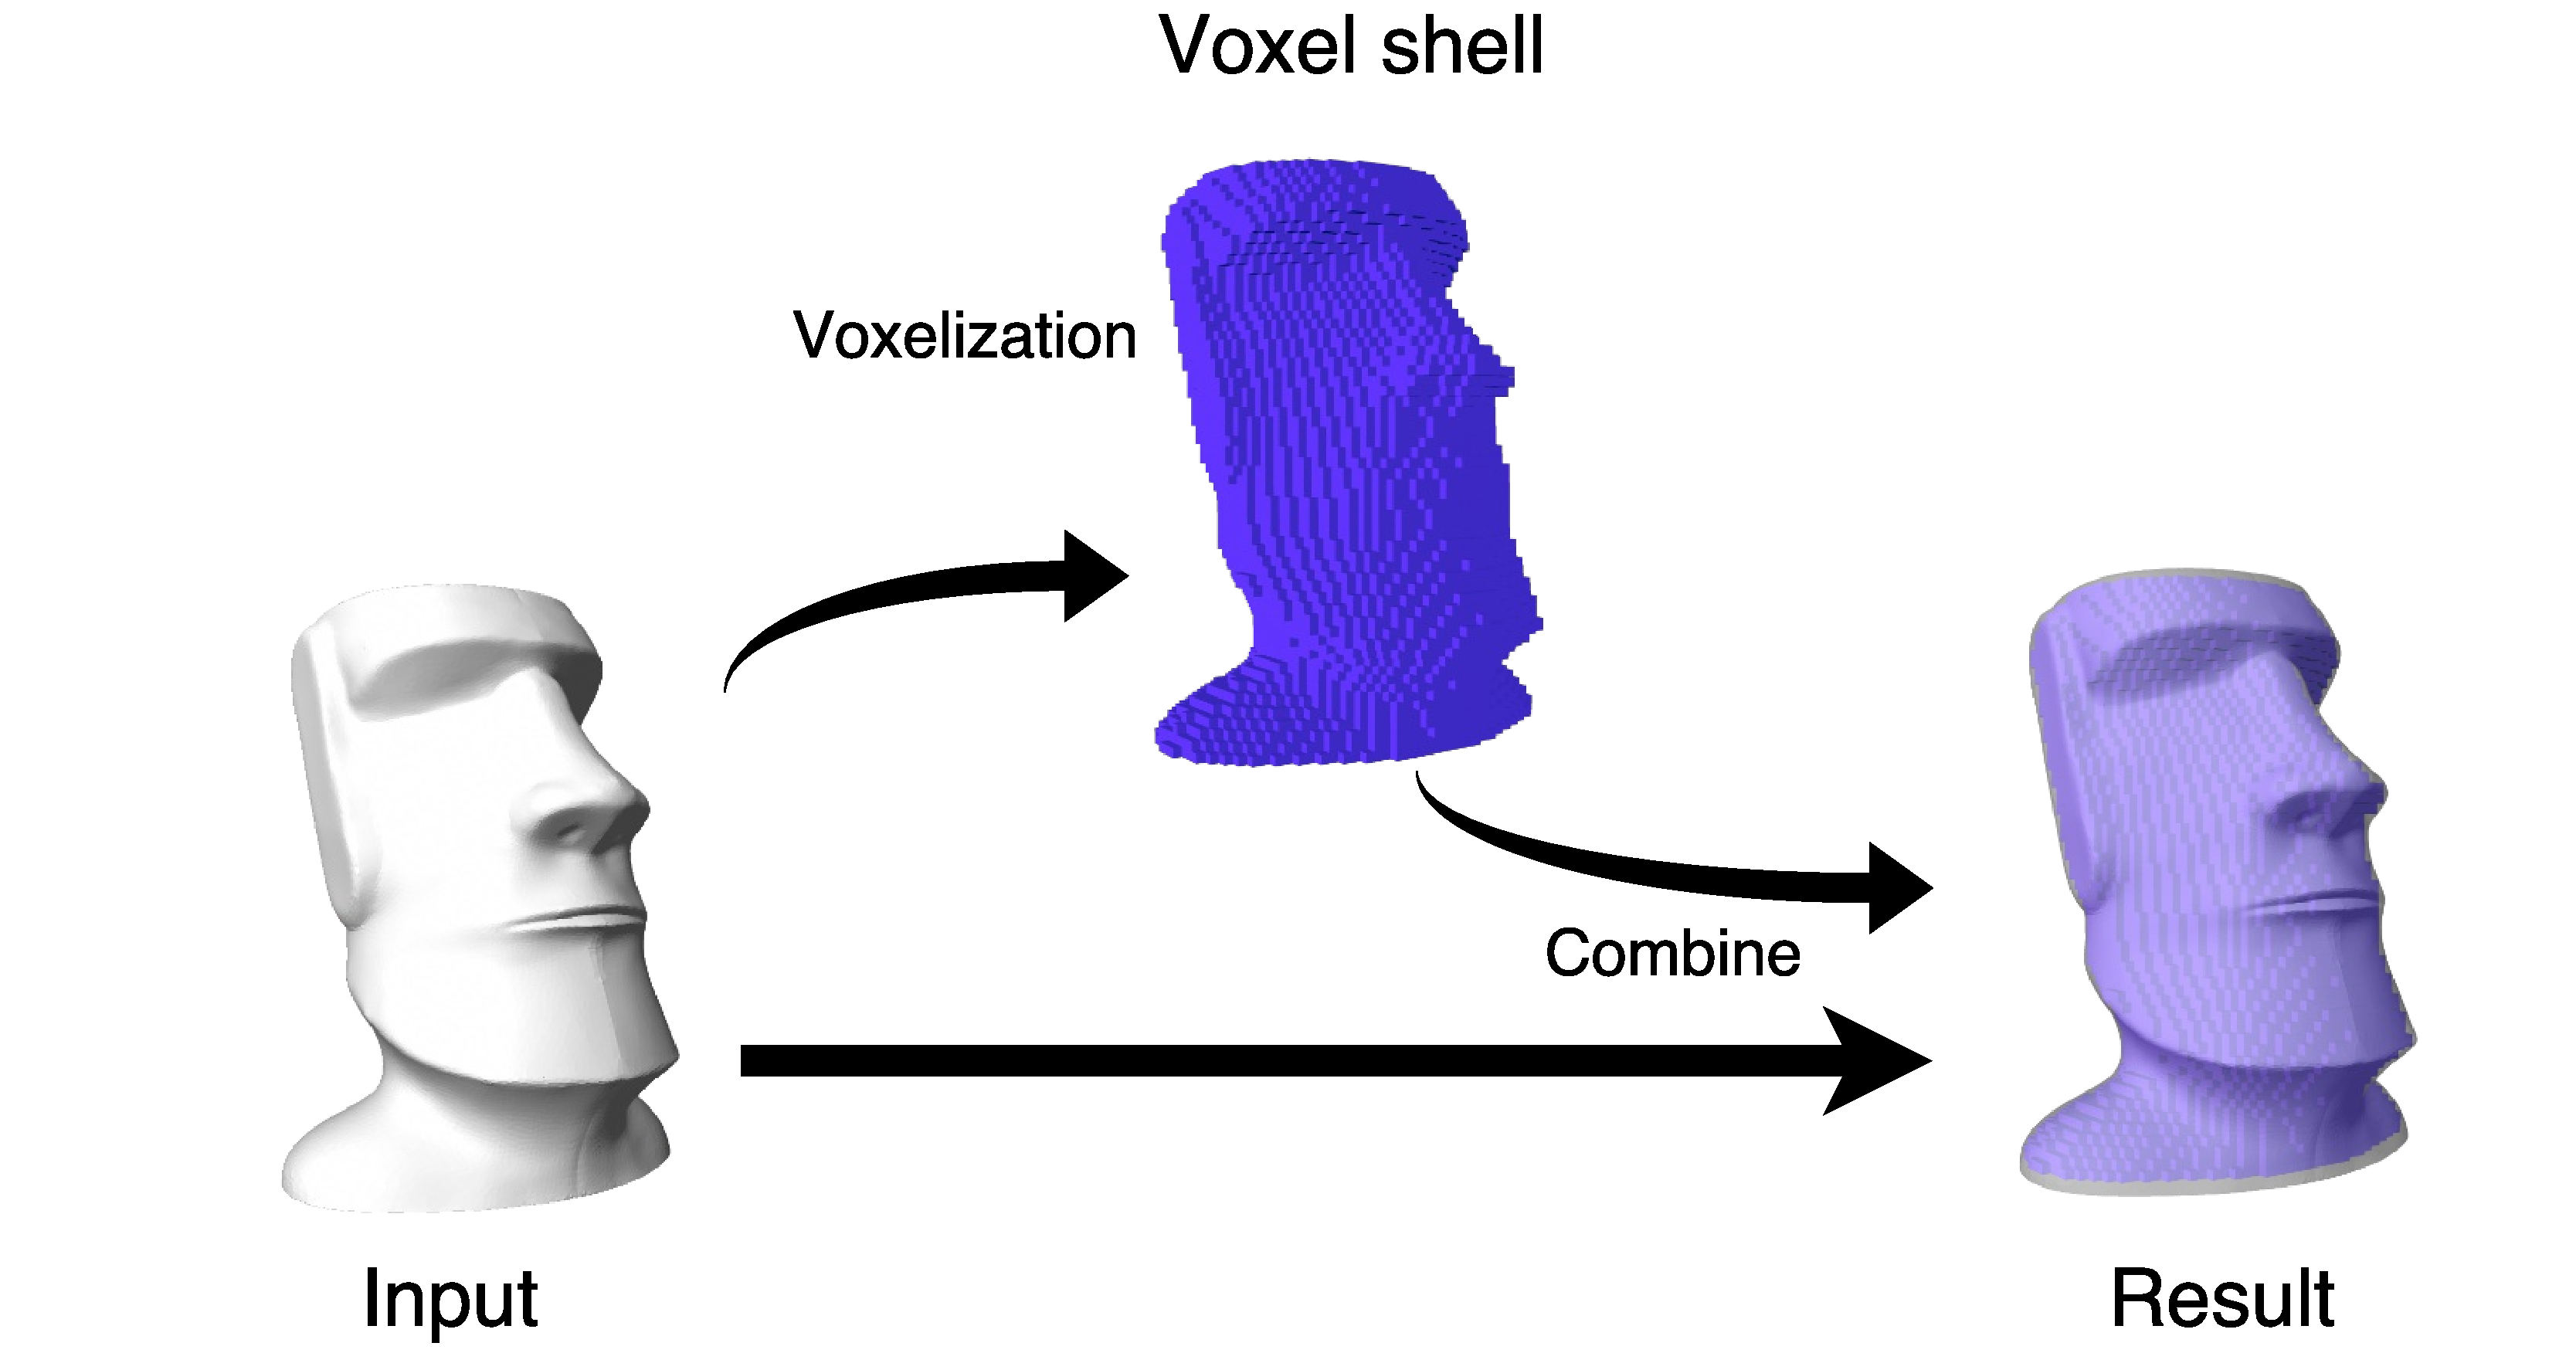
\includegraphics[width=1.0\linewidth]{figs/inner2.pdf} 
\caption{Inner surface generation method.}
\label{fig:inner_surface}
\end{figure}

% \subsection{Split mesh}
% In order to let user assemble the pieces easily, we use planar-cut method for mesh segmentation and find out the cut-plane in previous chapter. (see \secname ~\ref{sec:surf_part}) Then, we reference the function in open source software Blender~\cite{BLD} and modify it to be able to handle multiple plane cut. The alternative method help us get the segments, but the segments still can't be printed because of the hole between the outer and inner surface. We check each plane and find the vertices which align the plane. The vertex cluster can create a face which can fill the hole. But 3{D} printer just can print the mesh constructed by triangle. So, the new faces need to triangulate then the segment finally can be printed by the 3{D} printer. The details of split mesh process are in \figname~\ref{fig:split}.

% \begin{figure}[ht]
% \centering
% 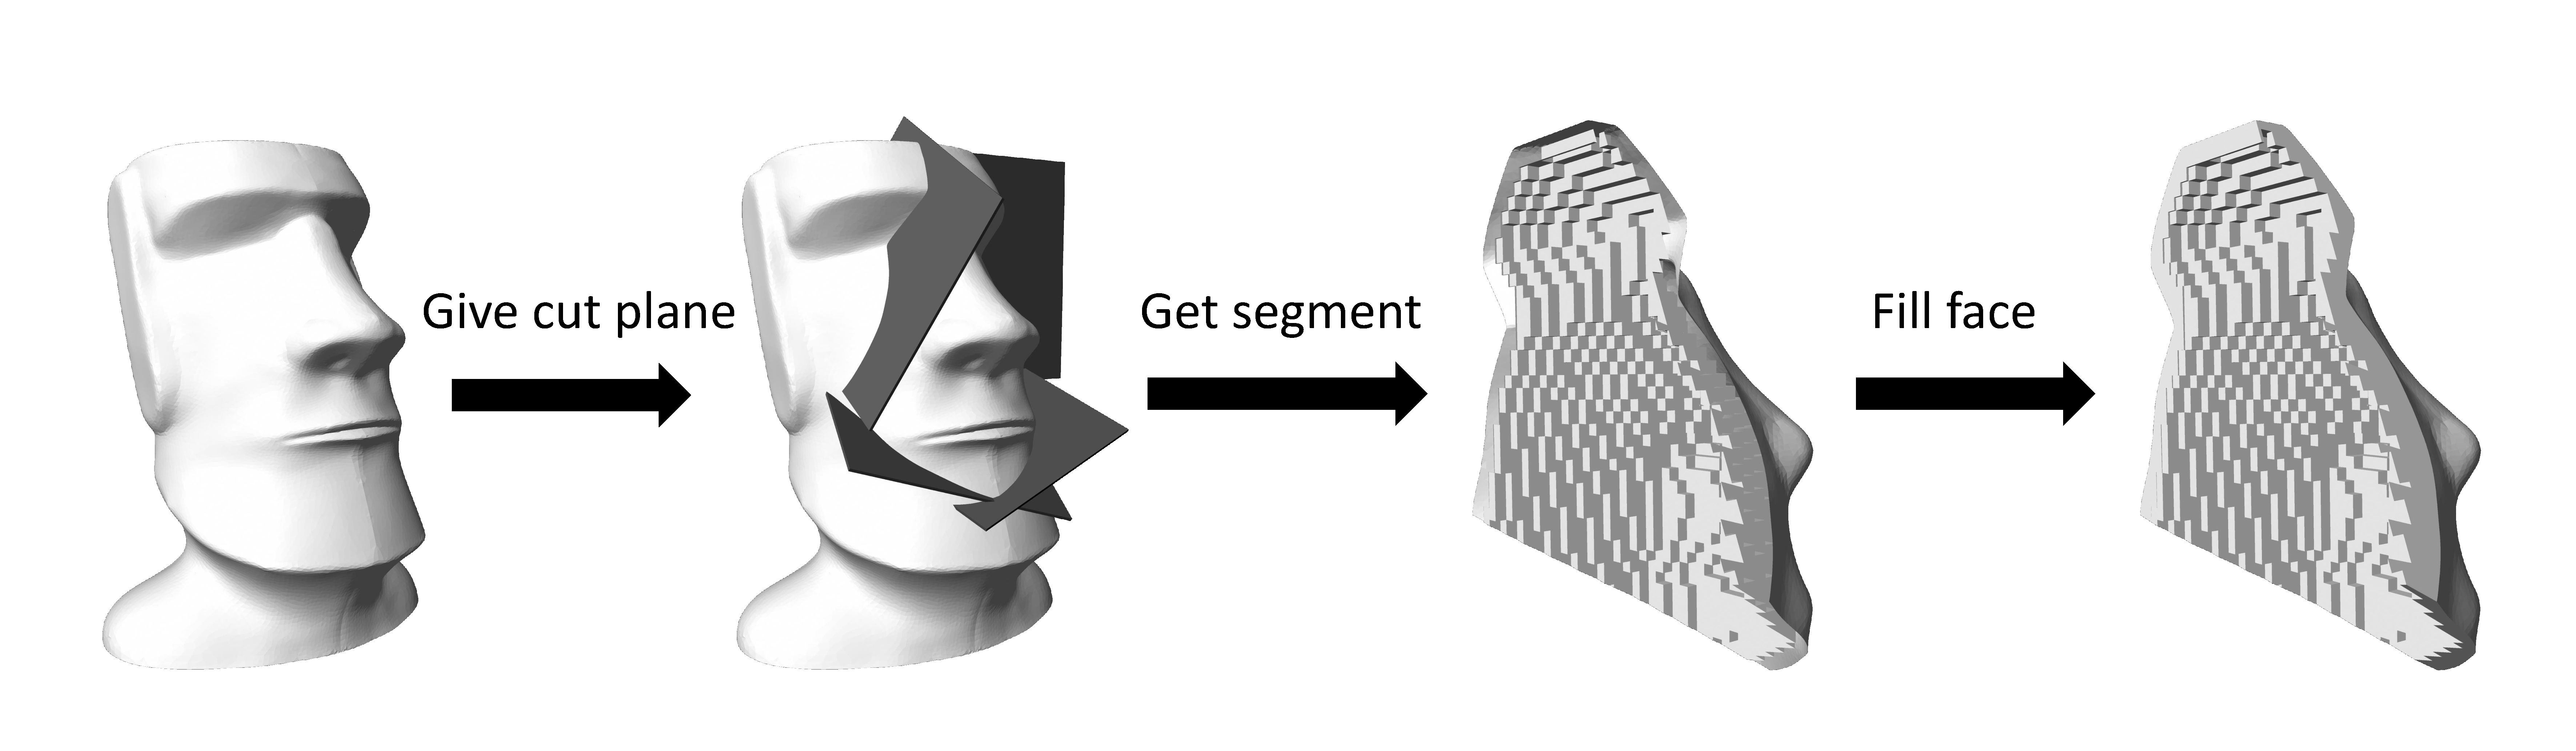
\includegraphics[width=1.0\linewidth]{figs/split.pdf} 
% \caption{Split mesh process.}
% \label{fig:split}
% \end{figure}
    
\subsection{Generate connector}
%After get the inner surface, we are able to use the partitioned results from graph cut to cut the surface into pieces. 
With the inner surface, we need to place connectors on it to connect between inner Zometool structure and outer shells.
% After get the split pieces, we need to connect the inner Zometool surface with these cutting pieces.
% But the pieces have to generate some connection to connect the inner Zometool structure. 
Two potential designs for building these connectors are:
\begin{enumerate}
\item Dig holes on the surface and use the Zometool rods to connect both inner and outer structure (\figname~\ref{fig:exp_surface_dig}).
\item  Grow Zometool tenons on the surface instead (\figname~\ref{fig:exp_surface_tenon}).
\end{enumerate}
We will elaborate how we implement both designs and discuss the pros and cons of both designs in the following paragraph.
% The following context will discuss more detail.
% For example, the connection can dig some holes on the surface and use the Zometool rod to connect the structure.(in Fig 4 (a)). 
% The other method is grow Zometool tenons on the surface.(in Fig 4 (b)) 
\subsubsection{Dig holes}
As observed, naively digging holes on the inner surface is likely to break the outer surface.
Instead, we have to grow additional structure that replicate Zome-ball, which is called ``virtual ball'' on the inner surface.
And we dig holes on this virtual ball to connect with Zometool structure using zometool struts.
However, as the objects usually printed with support materials generated by 3D printer, we observed that these support materials will greatly reduce the quality of these holes.
The major reason is that the holes are filled with the support materials and it is really hard to clean all of them.
As a result, the Zometool struts can not be inserted well (\figname~\ref{fig:exp_surface_dig} (b)).
To address this issue, practically we can change the printing directions, e.g. place the holes face upward to the printing plate so that no support materials will be printed inside the holes.
However, this means that the outer surface is attached to the support materials, and the final printed appearance will be pretty poor.
The issue can not be handled well given the limited precision of consumer-level 3D printer.
Hence, we propose an alternative connector design.
% If we want to dig some connecting holes on surface, we can't directly dig it because it might break the outer surface.
% To deal with it, the inner surface have to grow additional materials for digging. 
% We put a new Zome-ball called "virtual ball" on the inner surface which can have the additional materials for digging holes. 
% Then we can dig the holes on the virtual ball, thus the outer shell will not be broken. 
% The rods can use holes for connecting the main structure. 
% The downside of this approach is that shapes are usually printed with support materials, and the dug hole are usually filled with these materials. 
% If the support don't clean very well, the Zometool rods can't insert it. (see \figname~\ref{fig:exp_surface_dig}(b)) 
% In order to prevent the support material from generating in the holes during printing, we have to place the holes face upward to the printing plate. 
% The part which attaches the support materials always have worse quality. The holes face upward to the printing plate means that the outer surface is attached by the support materials, the final assembled result quality will be very poor.
% However, 3{D} printing can't print without the support material, the dig hole will fill with support material. 
% Due to the low precision issues for most of the consumer 3D printers, it is impractical to generate clean holes for Zometool tenon to plug in.
% Hence, we design an alternative approch to generate the connectors.
% If we don't clean the support clearly, the Zometool rod can't insert it. Beside, Zometool tenon is very small, the holes we dig are also small. The support material is very difficult to clean clearly. So we give up this method.
    
\subsubsection{Grow tenons on surface}
Zometool's tenon is a very small object, it fit perfectly on the Zome-ball and make the structure pretty robust. 
However, the size of tenon is a strong challenge for the 3{D} printer due to it's limited precision. 
Beside, same object will be printed differently under different orientations because the way of support printing.
In order to verify our 3{D} printer (Ultimaker 3 \footnote{https://ultimaker.com/en/products/ultimaker-3}) is able to print the tenons, we design an exhaustive experiment as follow:
we use Ultimaker 3 to print three different tenon of Zometool (rectangle, pentagon, triangle), each print in twenty-seven directions. 
As a result, we found out that even under the lowest precision (``fast print'' mode in Ultimaker 3), the printed tenons can still perfectly fit into the slots on the Zometool balls.
Compared to dig holes on surface, it is also easier to clean the printed support materials on the printed tenons.
Given it's easier clean up and more robust structure, we use this design to connect the inner Zometool structure and outer shells. 

And we decide how many tenons on each outer shell with following process:
We shoot rays from each slot on a single Zome-balls in the optimized Zometool structure $\mathbf{S}$, and record whether it intersect with the surface.
We repeat this examination on all of the 62 slots on the Zome-balls, and we grow tenons on the surface along the direction with the most ray-surface intersections.
% Finally, we grow tenons on surface 
% We search the nearest node on inner Zometool structure on split piece by graph cut for each triangle. 
% There are sixty-two slots on the Zome-ball, it means we can get sixty-two directions to grow the tenons. 
% We choose the direction which can grow most tenons on the surface to make a strong connection on the inner Zometool structure.

% \subsubsection{Discussion}
% \textbf{Dig holes} and \textbf{Grow tenons on surface} are two different methods for generating connection to the main inner structure. Each of method has disadvantages. \textbf{Dig holes} has problems of cleaning support material and quality. \textbf{Grow tenons on surface} has a problem that sometimes the tenons are broken when user clean up the printing support. The reason is the connection place will get the weak structure during slicer for 3D printing if we just insert the tenons mesh on surface directly. In order to reinforce the structure, we use CSG operation to combine the surface and tenons structure. Then the combine results are very robust. Our method want to approach \textbf{generating easily} and \textbf{good quality}. The problem of \textbf{Dig holes} are opposite to our main goal. So, we choose \textbf{Grow tenons on surface} for our generating connection to the main inner structure. 
    
\begin{figure}[ht]
\centering
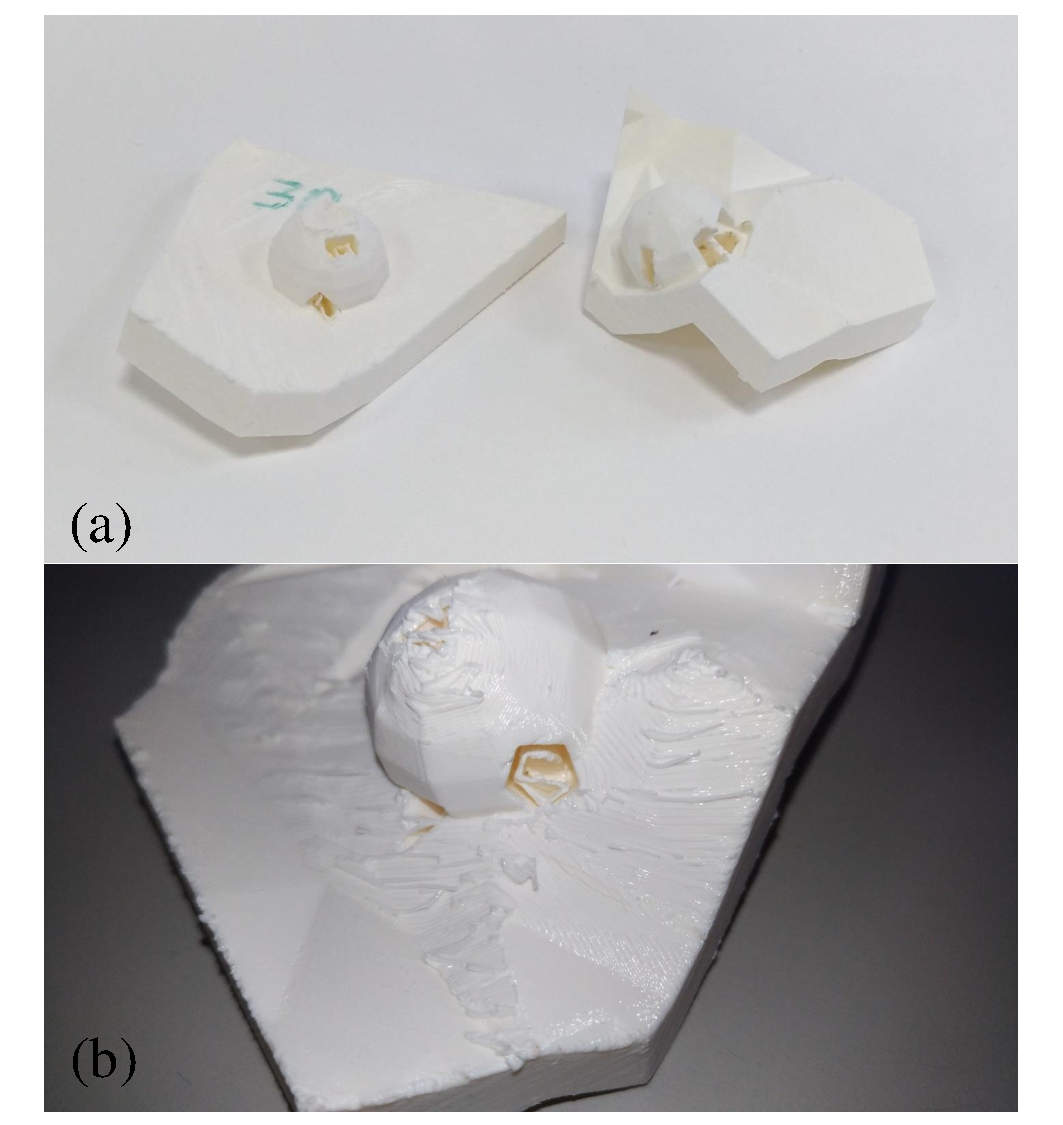
\includegraphics[width=1.0\linewidth]{figs/dig_hole.pdf} 
\caption{Experiment: Dig holes on inner surface (a) result (b)  support materials can't be cleaned well}
\label{fig:exp_surface_dig}
\end{figure}

\begin{figure}[ht]
\centering
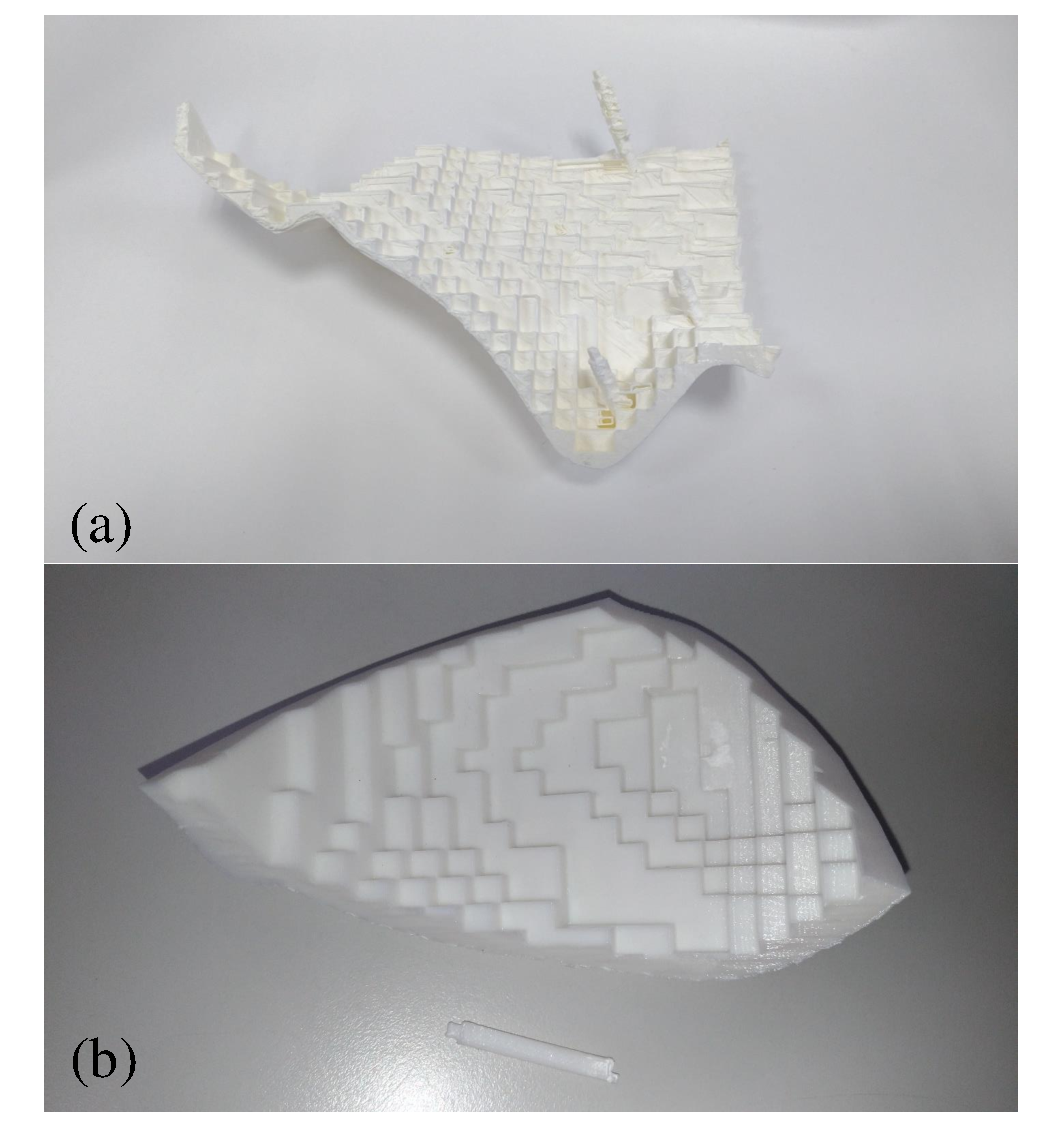
\includegraphics[width=1.0\linewidth]{figs/grow_tenon.pdf} 
\caption{Experiment: Grow tenons on surface (a) result (b) tenons broken}
\label{fig:exp_surface_tenon}
\end{figure}
